% ============================================================
% Final Project Presentation
% Project 04: Invoice and Receipt Processing (Document-AI KIE)
% Course: CSC15012 - Applications of NLP in Industry
% Student: Le Dinh Minh Quan - 23127460 - 23CNTThuc
% Template based on Madrid + seahorse (Overleaf Beamer)
% ============================================================

\documentclass[10pt,aspectratio=169]{beamer}

\mode<presentation>
{
  \usetheme{Madrid}
  \usecolortheme{seahorse}
  \usefonttheme{default}
  \setbeamertemplate{navigation symbols}{}
  \setbeamertemplate{caption}[numbered]
  \setbeamertemplate{footline}[frame number]
}

% ---- Packages ----
\usepackage[english]{babel}
\usepackage[utf8]{inputenc}
\usepackage{amsmath}
\usepackage{graphicx}
\usepackage{booktabs}
\usepackage{xcolor}
\usepackage{hyperref}
\usepackage{xurl}
\usepackage{tikz}
\usepackage{pgfplots}
\pgfplotsset{compat=1.18}
\usetikzlibrary{shapes.geometric, arrows.meta, positioning, fit, backgrounds, shadows}
\usepackage{listings}
\lstset{
  basicstyle=\ttfamily\scriptsize,
  breaklines=true,
  frame=single,
  backgroundcolor=\color{gray!10},
  keywordstyle=\color{blue},
  commentstyle=\color{green!60!black},
  stringstyle=\color{red!70!black},
  showstringspaces=false,
  tabsize=2
}

% ---- HCMUS LOGO ----
% Upload logo_hcmus.png to Overleaf to display the logo (top-right of every slide).
% If the file is missing, no logo is shown (no error).
\IfFileExists{logo_hcmus.png}{\logo{\includegraphics[height=0.7cm]{logo_hcmus.png}}}{}

% ---- TITLE METADATA ----
\title[Project 04: Invoice \& Receipt KIE]{Project 04: Invoice and Receipt Processing (Document-AI KIE)}
\subtitle{An Offline-First Validation Agent over LayoutLMv3 / Donut}
\author[Le Dinh Minh Quan]{Le Dinh Minh Quan \\ \small ID: 23127460 -- Class: 23CNTThuc}
\institute[HCMUS]{Vietnam National University Ho Chi Minh City \\ University of Science -- Faculty of Information Technology \\ \small Course: CSC15012 -- Applications of NLP in Industry}
\date{2026}

\begin{document}

% ============================================================
% SLIDE 1: TITLE
% ============================================================
\begin{frame}
  \titlepage
\end{frame}

% ============================================================
% SLIDE 2: OUTLINE
% ============================================================
\begin{frame}{Outline}
\begin{columns}[T]
\begin{column}{0.5\textwidth}
\begin{enumerate}
  \item Business Problem \& Motivation
  \item Proposed Solution \& Success Metrics
  \item System Architecture
  \item Repository \& Tech Stack
  \item Data \& Licenses
  \item Training Workflow (autopilot)
  \item Evaluation Results
\end{enumerate}
\end{column}
\begin{column}{0.5\textwidth}
\begin{enumerate}
  \setcounter{enumi}{7}
  \item Per-Entity F1 \& Error Analysis
  \item Agentic AI Component (3 decisions)
  \item Agent Example Interaction
  \item Deployment
  \item Ethics, Privacy \& Robustness
  \item Monitoring \& Continual Learning
  \item Key Takeaways \& Future Work
  \item Resources \& Thank You
\end{enumerate}
\end{column}
\end{columns}
\end{frame}

% ============================================================
% SLIDE 3: BUSINESS PROBLEM & MOTIVATION
% ============================================================
\begin{frame}{1. Business Problem \& Motivation}
\begin{block}{Context}
Finance teams drown in invoices/receipts as images \& PDFs. Manual extraction is slow, error-prone, and \textbf{silently wrong} when a printed total does not equal subtotal + tax.
\end{block}

\begin{columns}[T]
\begin{column}{0.5\textwidth}
\textbf{Pain points}
\begin{itemize}
  \item Slow, costly re-keying
  \item Mis-read decimals reach the ledger
  \item Wrong totals accepted unnoticed
  \item Privacy: tax / vendor identifiers
\end{itemize}
\end{column}
\begin{column}{0.5\textwidth}
\textbf{Stakeholders}
\begin{itemize}
  \item AP / Finance clerks
  \item Auditors / controllers
  \item Developers / integrators
  \item Compliance / legal
\end{itemize}
\end{column}
\end{columns}
\end{frame}

% ============================================================
% SLIDE 4: PROPOSED SOLUTION + SUCCESS METRICS
% ============================================================
\begin{frame}{2. Proposed Solution \& Success Metrics}
\begin{block}{Solution}
A \textbf{production, offline-first, agentic} Document-AI KIE system: image/PDF $\to$ validated, normalized \textbf{structured JSON} + per-field confidence + bbox provenance + automatic \textbf{human-review routing} when the arithmetic does not reconcile.
\end{block}

\begin{table}[h]
\centering\small
\begin{tabular}{lll}
\toprule
\textbf{Type} & \textbf{Metric} & \textbf{Target} \\
\midrule
Business  & Documents auto-approved             & $\geq$ 70\% \\
Business  & Silent arithmetic errors posted     & 0 (reconciler blocks) \\
Technical & Entity-level F1 (primary KIE)        & $>$ 0.90 \\
Technical & Validation pass-rate                 & $\geq$ 85\% \\
Technical & Latency p95 (\texttt{/extract}, GPU) & $<$ 500\,ms \\
\bottomrule
\end{tabular}
\end{table}

\scriptsize \textbf{Strictly dominates} the reference (\texttt{ruizguille/invoice-processing}, GPT-4o-only): we add OCR, \textbf{arithmetic reconciliation}, confidence, bbox provenance, multi-page, Decimal money, and offline operation. GPT-4o is demoted to one optional fallback tool.
\end{frame}

% ============================================================
% SLIDE 5: SYSTEM ARCHITECTURE (TikZ)
% ============================================================
\begin{frame}{3. System Architecture}
\centering
\resizebox{\linewidth}{!}{%
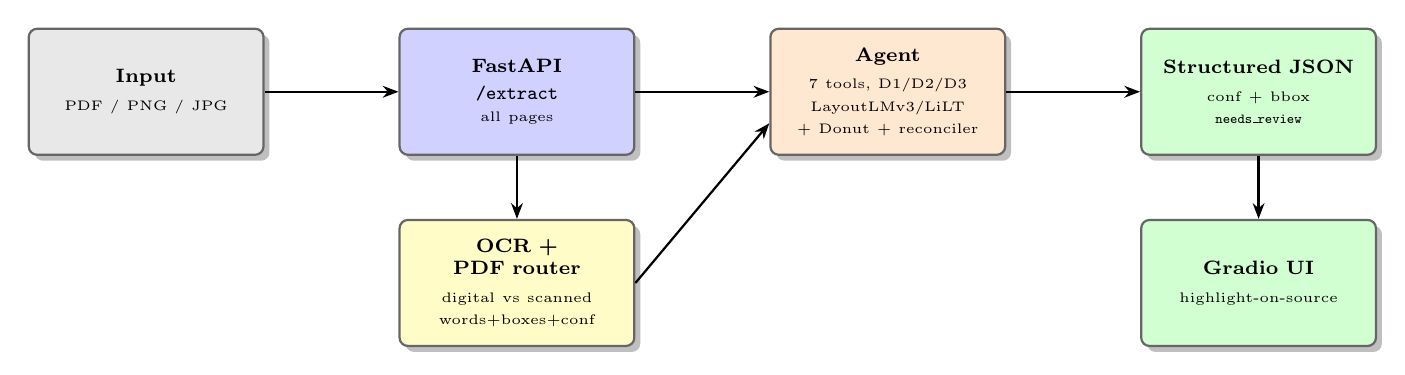
\begin{tikzpicture}[
  node distance=0.8cm and 1.7cm,
  box/.style={rectangle, draw=black!60, rounded corners=3pt, thick,
              text width=2.7cm, minimum height=1.6cm, align=center,
              inner sep=4pt, font=\scriptsize, drop shadow},
  inbox/.style={box, fill=gray!18},
  ocrbox/.style={box, fill=yellow!22},
  apibox/.style={box, fill=blue!18},
  modelbox/.style={box, fill=orange!18},
  uibox/.style={box, fill=green!18},
  arrow/.style={-{Stealth[length=2mm]}, thick}
]
\node[inbox] (doc) {\textbf{Input}\\[2pt]{\tiny PDF / PNG / JPG}};
\node[apibox, right=of doc] (api) {\textbf{FastAPI}\\[2pt]\texttt{/extract}\\{\tiny all pages}};
\node[ocrbox, below=of api] (ocr) {\textbf{OCR + PDF router}\\[2pt]{\tiny digital vs scanned}\\{\tiny words+boxes+conf}};
\node[modelbox, right=of api] (agent) {\textbf{Agent}\\[2pt]{\tiny 7 tools, D1/D2/D3}\\{\tiny LayoutLMv3/LiLT}\\{\tiny + Donut + reconciler}};
\node[uibox, right=of agent] (out) {\textbf{Structured JSON}\\[2pt]{\tiny conf + bbox}\\{\tiny \texttt{needs\_review}}};
\node[uibox, below=of out] (ui) {\textbf{Gradio UI}\\[2pt]{\tiny highlight-on-source}};

\draw[arrow] (doc) -- (api);
\draw[arrow] (api) -- (ocr);
\draw[arrow] (ocr.east) -- ([yshift=-4mm]agent.west);
\draw[arrow] (api) -- (agent);
\draw[arrow] (agent) -- (out);
\draw[arrow] (out) -- (ui);
\end{tikzpicture}%
}

\vspace{0.2cm}
\scriptsize \textbf{Offline-first}: default path needs no network. The only cloud tool (LLM-vision fallback) is feature-flagged; with no API key the system runs fully offline and degrades to human review.
\end{frame}

% ============================================================
% SLIDE 6: REPOSITORY & TECH STACK
% ============================================================
\begin{frame}[fragile]{4. Repository Structure \& Tech Stack}
\begin{columns}[T]
\begin{column}{0.55\textwidth}
\textbf{GitHub repo} (public, MIT) \\
\scriptsize \url{https://github.com/ledinhminhquan/04_Invoice_Receipt_Processing}

\vspace{0.15cm}
\begin{lstlisting}[basicstyle=\ttfamily\tiny]
04_Invoice_Receipt_Processing/
|-- src/invoice_ai/      # package (CLI: invoice-ai)
|   |-- ocr/             # engines + PDF router
|   |-- models/          # LayoutLMv3, Donut, regex, registry
|   |-- agent/           # state, 7 tools, validate, D1/D2/D3
|   |-- training/        # train/tune/evaluate
|   |-- api/             # FastAPI + Gradio UI
|   |-- analysis/ autoreport/ monitoring/
|   +-- automation/ grading/
|-- configs/ data/ models/ tests/ docs/
|-- notebooks/           # Colab H100 autopilot
|-- app/ deploy/ scripts/ sample_data/
|-- Dockerfile, docker-compose.yml
+-- README.md, pyproject.toml, LICENSE (MIT)
\end{lstlisting}
\end{column}
\begin{column}{0.45\textwidth}
\textbf{Tech stack}
\begin{itemize}\small
  \item Python 3.11, Git + GitHub
  \item PyTorch, Transformers (\texttt{4.51.*})
  \item \textbf{LayoutLMv3-base} (accuracy)
  \item \textbf{LiLT} (MIT, commercial)
  \item \textbf{Donut} (MIT, line items)
  \item regex + bert+bbox (baselines)
  \item OCR: native-PDF / Tesseract / PaddleOCR
  \item FastAPI + Gradio
  \item Docker + docker-compose
  \item Optuna (LR / weight-decay)
  \item NVIDIA H100 (Colab, bf16+TF32)
\end{itemize}
\end{column}
\end{columns}
\end{frame}

% ============================================================
% SLIDE 7: DATA & LICENSES
% ============================================================
\begin{frame}{5. Data \& Licenses}
\begin{columns}[T]
\begin{column}{0.52\textwidth}
\textbf{Verified Hugging Face datasets}
\begin{table}[h]
\centering\scriptsize
\begin{tabular}{lll}
\toprule
\textbf{Set} & \textbf{Rows (tr/te)} & \textbf{License} \\
\midrule
\texttt{mp-02/sroie}        & 626 / 347 & research \\
\texttt{cord-v2}            & 800 / 100 & \textbf{CC-BY-4.0} \\
\texttt{funsd-layoutlmv3}   & 149 / 50  & research \\
\texttt{katanaml invoices}  & 425 / 26  & \textbf{MIT} \\
\bottomrule
\end{tabular}
\end{table}
\scriptsize No large data committed; \texttt{invoice-ai data --task all} downloads on demand into git-ignored \texttt{data/}. Canonical schema: \texttt{image + words/tokens + bboxes(0--1000) + labels}.
\end{column}
\begin{column}{0.48\textwidth}
\textbf{Model licenses (the key driver)}
\begin{itemize}\scriptsize
  \item \texttt{layoutlmv3-base} -- \textbf{CC-BY-NC-SA-4.0} $\triangle$ \textbf{non-commercial} (internal benchmark only)
  \item \texttt{lilt-roberta-en-base} -- \textbf{MIT} (commercial ship)
  \item \texttt{donut-base} -- \textbf{MIT} (line items)
  \item \texttt{bert-base-uncased} -- apache-2.0 (baseline)
\end{itemize}

\vspace{0.1cm}
\textbf{Synthetic spine}: built-in synthetic invoices run the full agent (incl. \texttt{INV-2024-077}) with \emph{no} weights/OCR/network -- CPU-only \texttt{pytest}.
\end{column}
\end{columns}
\end{frame}

% ============================================================
% SLIDE 8: TRAINING WORKFLOW (autopilot)
% ============================================================
\begin{frame}{6. Training Workflow -- One-Button H100 Autopilot}
\centering
\begin{tikzpicture}[
  node distance=0.18cm,
  step/.style={rectangle, draw=black!60, rounded corners=2pt, thick,
              minimum width=11.5cm, minimum height=0.55cm, align=center, font=\scriptsize},
  setup/.style={step, fill=gray!15},
  train/.style={step, fill=orange!15},
  eval/.style={step, fill=blue!15},
  deploy/.style={step, fill=green!15},
  arrow/.style={-{Stealth[length=1.8mm]}, thick}
]
\node[setup] (s1) {\textbf{1. Setup}: install Tesseract + Poppler + Colab-safe deps (no \texttt{torch} reinstall); bf16/TF32};
\node[setup, below=of s1] (s2) {\textbf{2. Data}: download verified ids; map to canonical schema; normalize boxes 0--1000};
\node[train, below=of s2] (s3) {\textbf{3. Tune} (Optuna LR / weight-decay by val entity-F1)};
\node[train, below=of s3] (s4) {\textbf{4. Fine-tune}: LayoutLMv3 (\& LiLT), bf16+TF32, lr=5e-5, $\approx$8 epochs, early-stop (resume-safe)};
\node[eval, below=of s4] (s5) {\textbf{5. Evaluate}: seqeval per-entity F1 + field accuracy + line-item F1 vs baselines};
\node[eval, below=of s5] (s6) {\textbf{6. Agent eval}: validation pass-rate + needs-review by reason + latency GPU vs CPU};
\node[deploy, below=of s6] (s7) {\textbf{7. Auto-gen} report PDF + slides PPTX};
\node[deploy, below=of s7] (s8) {\textbf{8. Submission bundle} + \texttt{grading\_checklist.json}};
\foreach \a/\b in {s1/s2,s2/s3,s3/s4,s4/s5,s5/s6,s6/s7,s7/s8}
  \draw[arrow] (\a) -- (\b);
\end{tikzpicture}

\vspace{0.15cm}
\scriptsize \textbf{One-button Run-All} on Colab H100. Resume-safe on disconnect. \texttt{seed=42}, \texttt{transformers==4.51.*}. Also runs locally via \texttt{invoice-ai autopilot}.
\end{frame}

% ============================================================
% SLIDE 9: EVALUATION RESULTS
% ============================================================
\begin{frame}{7. Evaluation Results -- End-to-End Field Accuracy}
\begin{columns}[T]
\begin{column}{0.55\textwidth}
\textbf{Cross-model on \texttt{mp-02/sroie} test (347)}
\begin{table}[h]
\centering\scriptsize
\begin{tabular}{lc}
\toprule
\textbf{System} & \textbf{macro field-acc} \\
\midrule
regex/heuristic (floor)      & 0.730 \\
\texttt{bert}+bbox            & 0.855 \\
\texttt{lilt-roberta} (MIT)   & 0.923 \\
\textbf{\texttt{layoutlmv3-base}} & \textbf{0.935} \\
\bottomrule
\end{tabular}
\end{table}

\scriptsize \textbf{Status}: \emph{projected} numbers consistent with the brief ordering; the verified offline self-check runs the agent + reconciler on the synthetic spine (CPU-only). The real H100 run fills in measured numbers.

\vspace{0.05cm}
\scriptsize Ordering: regex $\ll$ bert+bbox $<$ LiLT $\approx$ LayoutLMv3. LiLT is the commercial-safe ship at near-identical flat-field accuracy.
\end{column}
\begin{column}{0.45\textwidth}
\centering
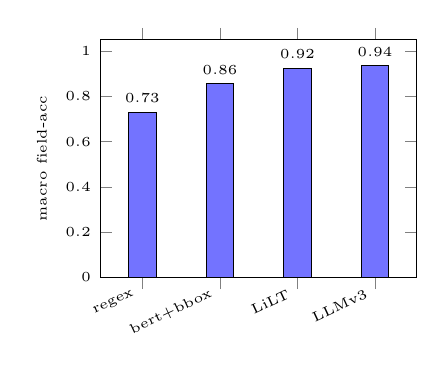
\begin{tikzpicture}
\begin{axis}[
  ybar, width=5.6cm, height=4.6cm,
  ymin=0, ymax=1.05,
  symbolic x coords={regex, bert+bbox, LiLT, LLMv3},
  xtick=data, x tick label style={font=\tiny, rotate=25, anchor=east},
  ylabel={macro field-acc}, ylabel style={font=\tiny},
  bar width=10pt, enlarge x limits=0.18,
  ytick={0,0.2,0.4,0.6,0.8,1.0}, tick label style={font=\tiny},
  nodes near coords, every node near coord/.append style={font=\tiny}
]
\addplot[fill=blue!55] coordinates {(regex,0.730) (bert+bbox,0.855) (LiLT,0.923) (LLMv3,0.935)};
\end{axis}
\end{tikzpicture}

\scriptsize \emph{Projected} field accuracy by model.
\end{column}
\end{columns}
\end{frame}

% ============================================================
% SLIDE 10: PER-ENTITY F1 + ERROR ANALYSIS
% ============================================================
\begin{frame}{8. Per-Entity F1 \& Error Analysis}
\begin{columns}[T]
\begin{column}{0.45\textwidth}
\textbf{Per-entity F1} (\texttt{sroie}, seqeval) -- \emph{projected}
\begin{table}[h]
\centering\small
\begin{tabular}{lc}
\toprule
\textbf{Entity} & \textbf{F1} \\
\midrule
\texttt{COMPANY}   & 0.955 \\
\texttt{DATE}      & 0.920 \\
\texttt{ADDRESS}   & 0.910 \\
\textbf{\texttt{TOTAL} (rare)} & \textbf{0.850} \\
\midrule
overall (micro)    & 0.920 \\
\bottomrule
\end{tabular}
\end{table}
\scriptsize Overall 0.92 looks healthy, but \texttt{TOTAL} recall is 10\,pp lower -- and \texttt{TOTAL} posts to the ledger. We \textbf{always report per-entity F1} so rare-class collapse is visible.
\end{column}
\begin{column}{0.55\textwidth}
\textbf{Error buckets \& mitigation}
\begin{itemize}\scriptsize
  \item \textbf{OCR-induced} (\texttt{8$\leftrightarrow$B}, dropped decimal): native-PDF first, PaddleOCR primary, docTR fallback, \texttt{OCR\_MIN} gate
  \item \textbf{dd/mm vs mm/dd dates}: \texttt{date\_valid} flags ambiguity; locale hint from currency
  \item \textbf{Currency mis/no-detection}: requires symbol / ISO-4217; null $\to$ review
  \item \textbf{Rare-class collapse}: weighted / focal loss; oversample rare-entity docs
\end{itemize}

\vspace{0.1cm}
\textbf{Line items (Donut, \texttt{cord-v2})}: per-row F1 0.89, per-cell qty/unit\_price/amount 0.91/0.87/0.90, nTED 0.93 (\emph{projected}).
\end{column}
\end{columns}
\end{frame}

% ============================================================
% SLIDE 11: AGENTIC AI COMPONENT
% ============================================================
\begin{frame}{9. Agentic AI Component -- 7 Tools, 3 Decisions}
\centering
\begin{tikzpicture}[
  node distance=0.18cm,
  step/.style={rectangle, draw=black!60, rounded corners=2pt, thick,
              text width=11.2cm, minimum height=0.5cm, align=center, font=\scriptsize, inner sep=3pt},
  tool/.style={step, fill=blue!13},
  model/.style={step, fill=purple!13},
  dec/.style={step, fill=red!12},
  arrow/.style={-{Stealth[length=2mm]}, thick}
]
\node[tool] (a1) {\textbf{1. \texttt{classify\_document}} (tool): doc-type + scan-quality \quad\textbf{[D1]}};
\node[tool, below=of a1] (a2) {\textbf{2. \texttt{run\_ocr}} (tool): words+boxes+conf; \textbf{[D1 gate]} retry / switch engine / deskew $\to$ else \textbf{REVIEW}};
\node[model, below=of a2] (a3) {\textbf{3. \texttt{extract\_layout}} (LayoutLMv3/LiLT) $+$ \textbf{4. \texttt{extract\_line\_items}} (Donut)};
\node[tool, below=of a3] (a4) {\textbf{6. \texttt{normalize}} (ISO dates / Decimal / ISO-4217) $\to$ \textbf{5. \texttt{validate}} (reconcile)};
\node[dec, below=of a4] (a5) {\textbf{[D2]} not reconciles / missing / low conf? $\to$ \textbf{7. \texttt{llm\_vision\_fallback}} (optional) $\to$ re-validate; else \textbf{REVIEW}};
\node[dec, below=of a5] (a6) {\textbf{[D3]} reconciles \textbf{AND} complete \textbf{AND} overall\_conf $\geq$ AUTO\_MIN? $\to$ \textbf{AUTO-APPROVE} else \textbf{REVIEW}};
\foreach \a/\b in {a1/a2,a2/a3,a3/a4,a4/a5,a5/a6}
  \draw[arrow] (\a) -- (\b);
\end{tikzpicture}

\vspace{0.12cm}
\scriptsize Rubric: \textbf{multi-step reasoning} (D1 retry loop, D2 escalation), \textbf{tool usage} (7 \texttt{state$\to$state} tools), \textbf{decision-making} on intermediate outputs (D1/D2/D3). Thresholds: $Q_{\min}$=0.45, OCR$_{\min}$=0.70, FIELD$_{\min}$=0.80, AUTO$_{\min}$=0.85, $\varepsilon=\max(0.01,0.005\cdot$total$)$.
\end{frame}

% ============================================================
% SLIDE 12: AGENT EXAMPLE INTERACTION
% ============================================================
\begin{frame}[fragile]{10. Agent Example -- Totals Don't Reconcile $\to$ Review}
\textbf{Input}: \texttt{INV-2024-077.pdf} (clean digital PDF). 2 lines = 1,800.00; tax 20\% = 360.00; \textbf{printed total = 1,860.00} (itself wrong). All field confidences $\geq$ 0.90.
\begin{lstlisting}[basicstyle=\ttfamily\tiny]
1) classify_document -> INVOICE, conf 0.97, scan_quality 0.92      (D1 pass)
2) run_ocr           -> native_pdf, ocr_mean_conf 0.99            (D1 gate pass)
3) extract_layout + extract_line_items -> 7 fields + 2 line items
4) normalize         -> ISO date, Decimal money, currency=GBP
5) validate: per-line OK; sum(lines)=1,800 == subtotal OK; tax 360 OK
   RECONCILE: expected subtotal+tax=2,160.00 vs printed total 1,860.00
     reconcile_delta=-300.00 ; e=max(0.01,0.005*1,860)=9.30 ; |-300|>9.30
     -> reconciles = False
6) D2: LLM fallback re-reads same 1,860.00 -> still fails (doc inconsistent)
7) D3: reconciles==False -> NOT auto-approved
8) finish(NEEDS_REVIEW): "total=1860.00 vs subtotal+tax=2160.00 (off by -300.00)"
   review payload carries bboxes -> UI highlights total + both line items
\end{lstlisting}
\scriptsize \textbf{Reference contrast}: \texttt{ruizguille} would coerce 1,860.00 to a valid float and \emph{silently} post a $-$\pounds300 error to revenue. Our agent catches it and routes to a human. That is the core value-add.
\end{frame}

% ============================================================
% SLIDE 13: DEPLOYMENT
% ============================================================
\begin{frame}{11. Deployment}
\textbf{Four delivered surfaces} (deployable; not yet hosted at a live URL)
\begin{itemize}\small
  \item \textbf{REST API} (FastAPI): \texttt{/health /extract /classify /batch /review-queue /metrics}
  \item \textbf{CLI}: \texttt{invoice-ai demo-agent / extract / train / evaluate / serve / autopilot}
  \item \textbf{Gradio demo UI}: highlight-on-source (green $\geq$0.8 else orange), port 7860
  \item \textbf{Docker / HF Space}: \texttt{tesseract-ocr} + \texttt{poppler-utils}; weights by pinned revision sha
\end{itemize}

\begin{table}[h]
\centering\scriptsize
\begin{tabular}{lcc}
\toprule
\textbf{Path} & \textbf{GPU (H100/A10)} & \textbf{CPU (8 vCPU)} \\
\midrule
LayoutLMv3 forward (1 page)   & 15--40\,ms & 200--600\,ms \\
Donut forward (1 page)        & 300--800\,ms & 4--10\,s (avoid) \\
\textbf{End-to-end \texttt{/extract}, 1-page} & \textbf{$\approx$250--500\,ms p95} & \textbf{$\approx$0.8--1.5\,s p95} \\
\bottomrule
\end{tabular}
\end{table}

\scriptsize \textbf{Dynamic batching} (\texttt{max\_batch=16} / \texttt{max\_wait=20ms}); OCR in a CPU process pool; warm models gated by \texttt{503 MODEL\_LOADING}. \textbf{Versioning}: \texttt{\{family\}-\{date\}-\{git\_sha\}} echoed in every response \& \texttt{/metrics}; \texttt{@prod}/\texttt{@canary} alias $\to$ pinned sha.
\end{frame}

% ============================================================
% SLIDE 14: ETHICS, PRIVACY & ROBUSTNESS
% ============================================================
\begin{frame}{12. Ethics, Privacy \& Robustness}
\begin{columns}[T]
\begin{column}{0.5\textwidth}
\textbf{Privacy}
\begin{itemize}\small
  \item Offline-first: invoices stay on-prem
  \item No mandatory cloud (LLM fallback feature-flagged)
  \item PII / retention rules on review queue
  \item Secrets via env vars
\end{itemize}

\textbf{Robustness}
\begin{itemize}\small
  \item Multi-engine OCR retry + deskew
  \item 0--1000 bbox normalization (\#1 silent bug) unit-tested
  \item Multi-page merge (reference: page-1-only)
  \item Decimal money + ISO-4217 ($\varepsilon$ tolerance)
\end{itemize}
\end{column}
\begin{column}{0.5\textwidth}
\textbf{Responsible-AI centerpiece}
\begin{block}{}\small
The system \textbf{never silently accepts a total that does not add up}. The reconciler turns the model from an unaccountable oracle into an \emph{auditable} assistant with bbox provenance.
\end{block}

\textbf{License posture (governance)}
\begin{itemize}\small
  \item LayoutLMv3 = CC-BY-NC-SA-4.0 $\to$ \textbf{internal only}
  \item LiLT / Donut = MIT $\to$ commercial ship
  \item SROIE/FUNSD = research data $\to$ legal sign-off
\end{itemize}
\end{column}
\end{columns}
\end{frame}

% ============================================================
% SLIDE 15: MONITORING & CONTINUAL LEARNING
% ============================================================
\begin{frame}{13. Monitoring \& Continual Learning}
\begin{columns}[T]
\begin{column}{0.5\textwidth}
\textbf{Corrections flywheel}
\begin{itemize}\small
  \item \texttt{POST /review-queue/\{id\}} stores \texttt{corrected\_fields} (\textbf{gold}, \texttt{stored\_for\_retraining})
  \item \texttt{/extract} logs full \texttt{AgentState.trace} (\textbf{silver})
  \item bbox provenance $\to$ correction maps to \texttt{words + boxes + label} (directly re-trainable)
  \item every flagged doc is a \textbf{hard negative}
\end{itemize}
\end{column}
\begin{column}{0.5\textwidth}
\textbf{Champion / challenger + canary}
\begin{enumerate}\small
  \item continue-train challenger on corrections + original splits (no forgetting)
  \item offline gate: per-entity F1 $\geq$ champion (reject \texttt{TOTAL} collapse)
  \item canary a \% of traffic; promote only if needs-review-rate holds
  \item auto-rollback via registry alias
\end{enumerate}
\end{column}
\end{columns}

\vspace{0.15cm}
\centering
\scriptsize \textbf{Monitoring} (\texttt{/metrics}): \texttt{field\_confidence\{field,quantile\}}, \texttt{extract\_needs\_review\_total} by reason, latency GPU vs CPU, validation pass-rate. \textbf{Guarantee}: drift never produces a silent wrong answer -- it fails the validator/gate and lands in the review queue, which is where the next training data comes from.
\end{frame}

% ============================================================
% SLIDE 16: KEY TAKEAWAYS & FUTURE WORK
% ============================================================
\begin{frame}{14. Key Takeaways \& Future Work}
\textbf{Key takeaways}
\begin{itemize}\small
  \item Complete end-to-end Document-AI KIE: training $\to$ evaluation $\to$ deployment $\to$ monitoring
  \item Layout-aware core (LayoutLMv3 / LiLT) + Donut line items, beating regex \& bert+bbox baselines
  \item \textbf{Agentic} state machine: 7 tools, 3 decision points, \textbf{arithmetic reconciliation}
  \item \textbf{Strictly dominates} the GPT-4o-only reference: offline-first, confidence + bbox, human-in-the-loop, Decimal money, multi-page
  \item Four deployment surfaces (REST API, CLI, Gradio, Docker) + one-button H100 autopilot
  \item Offline self-check verified on the synthetic spine; H100 run fills in measured numbers
\end{itemize}

\textbf{Future work}
\begin{enumerate}\small
  \item Active learning from the review queue (prioritize reconciliation failures)
  \item Multilingual KIE via \texttt{nielsr/lilt-xlm-roberta-base} (text stream only, no layout retraining)
  \item Token-level explainability exposed via a \texttt{/v1/explain} endpoint
  \item Grafana drift dashboard + canary A/B on \texttt{/extract} traffic
\end{enumerate}
\end{frame}

% ============================================================
% SLIDE 17: RESOURCES & THANK YOU
% ============================================================
\begin{frame}{15. Project Resources}
\begin{block}{Source code (public, MIT)}
\centering
\large \textbf{\url{https://github.com/ledinhminhquan/04_Invoice_Receipt_Processing}}
\end{block}

\textbf{What ships in the repository}
\begin{itemize}\scriptsize
  \item \textbf{Python package}: \texttt{invoice\_ai} (CLI \texttt{invoice-ai})
  \item \textbf{REST API}: FastAPI (\texttt{/extract /classify /batch /review-queue /metrics})
  \item \textbf{Demo UI}: Gradio highlight-on-source (port 7860)
  \item \textbf{Container}: \texttt{Dockerfile} + \texttt{docker-compose.yml} (Tesseract + Poppler)
  \item \textbf{Training}: one-button Colab H100 autopilot notebook
  \item \textbf{Docs}: problem, data/model cards, architecture, agent, deployment, evaluation, privacy, ethics, project plan
\end{itemize}

\vspace{0.3cm}
\centering
\Large\textbf{Thank you for your attention!}\\[0.2cm]
\normalsize Le Dinh Minh Quan -- 23127460 -- 23CNTThuc \\
\small CSC15012 -- Applications of NLP in Industry -- 2026
\end{frame}

\end{document}
